\chapter{Clasificacion}\label{Chapter3} 
% chktex-file 8
% chktex-file 12
% chktex-file 13
% chktex-file 44


El modelo de regresión lineal presentado en el capítulo \ref{Chapter3} asume que la variable de respuesta $Y$ es cuantitativa. Sin embargo, en muchas situaciones, la variable de respuesta es cualitativa. A menudo las variables cualitativas se denominan categóricas. Los enfoques para predecir respuestas cualitativas son proceso conocidos como clasificación, ya que implica asignar la observación a una categoría o clase. Por otro lado, frecuentemente los métodos utilizados para clasificación primero predicen la probabilidad de cada una de las categorías de una variable cualitativa, como base para realizar la clasificación. En este sentido, también se comportan como métodos de regresión.

\section{El entorno de clasificación}

Muchos de los conceptos encontrados en los capítulos anteriores, como el equilibrio entre sesgo y varianza, se transfieren al contexto de clasificación con solo algunas modificaciones debido a que $y_i$ ya no es numérica. Supongamos que se busca estimar $f$ basándose en observaciones de entrenamiento ${(x_1,y_1), \dots,(x_n,y_n)}$, donde ahora $y_1,...,y_n$ son cualitativas. El enfoque más común para cuantificar la precisión de nuestra estimación $\hat{f}$ es la tasa de error de entrenamiento, la proporción de errores que se cometen si se aplica la estimación $\hat{f}$ a las observaciones de entrenamiento:
\begin{equation}
\frac{1}{n}\sum_{i=1}^n I(y_i \neq \hat{y}_i)
\label{eq:2.8}
\end{equation}

Aquí $\hat{y}_i$ es la etiqueta de clase predicha para la $i$-ésima observación usando $\hat{f}$, y $I(y_i \neq \hat{y}_i)$ es una variable indicadora que equivale a 1 si $y_i \neq \hat{y}_i$ y cero si $y_i = \hat{y}_i$. Si $I(y_i \neq \hat{y}_i) = 0$ entonces la $i$-ésima observación fue clasificada correctamente por nuestro método de clasificación; de lo contrario fue mal clasificada. Por lo tanto, la ecuación \ref{eq:2.8} calcula la fracción de clasificaciones incorrectas. \\

La ecuación \ref{eq:2.8} se conoce como la tasa de error de entrenamiento porque se calcula basándose en los datos que se utilizaron para entrenar el clasificador. Como en el contexto de regresión, se está más interesado en las tasas de error que resultan de aplicar nuestro clasificador a observaciones de prueba que no se utilizaron en el entrenamiento. La tasa de error de prueba asociada con un conjunto de observaciones de prueba de la forma $(x_0,y_0)$ está dada por:
\begin{equation}
\text{AVE}(I(y_0 \neq \hat{y}_0))
\label{eq:2.9}
\end{equation}

donde $\hat{y}_0$ es la etiqueta de clase predicha que resulta de aplicar el clasificador a la observación de prueba con predictor $x_0$. Un buen clasificador es aquel para el cual el error de prueba (\ref{eq:2.9}) es mínimo. \\

\subsection{El clasificador de Bayes}

Se puede demostrar que la tasa de error de prueba dada en (\ref{eq:2.9}) se minimiza, en promedio, por un clasificador muy simple que asigna cada observación a la clase más probable, dados sus valores de predictores. En otras palabras, se debe simplemente asignar una observación de prueba con vector de predictores $x_0$ a la clase $j$ para la cual 
\begin{equation}
\Pr(Y = j | X = x_0)
\label{eq:2.10}
\end{equation}

es mayor. Nótese que (\ref{eq:2.10}) es una probabilidad condicional: es la probabilidad de que $Y = j$, dado el vector de predictores observado $x_0$. Este clasificador tan simple se llama clasificador de Bayes. En un problema de dos clases donde solo hay dos posibles valores de respuesta, digamos clase 1 o clase 2, el clasificador de Bayes corresponde a predecir la clase uno si $\text{Pr}(Y = 1 | X = x_0) > 0.5$, y la clase dos en caso contrario. \\

\begin{figure}[h]
\centering
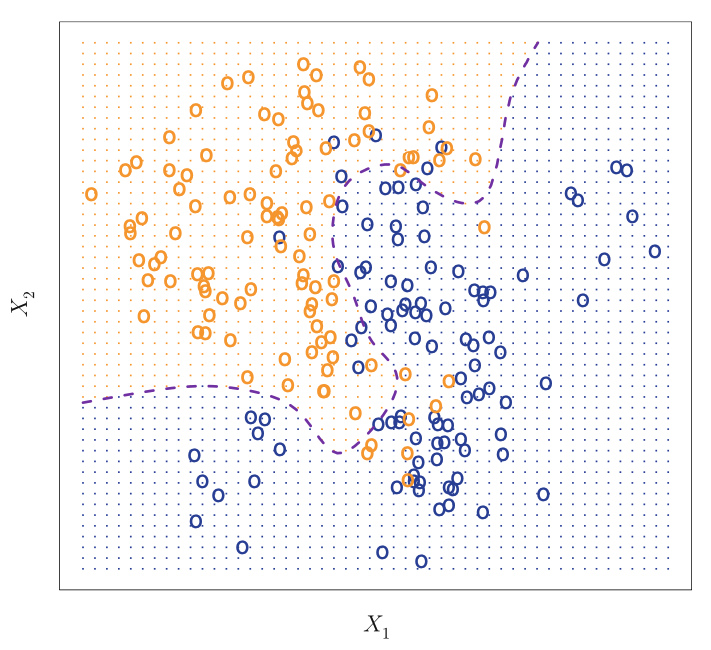
\includegraphics[width=0.6\textwidth]{fotos/9.png}
\caption{Conjunto de datos simulado de 100 observaciones en cada uno de los dos grupos, indicados en azul y en naranja. La línea discontinua púrpura representa la frontera de decisión de Bayes. La cuadrícula de fondo naranja indica la región en la cual una observación de prueba será asignada a la clase naranja, y la cuadrícula de fondo azul indica la región en la cual una observación de prueba será asignada a la clase azul.}
\label{fig:2.13}
\end{figure}

La figura \ref{fig:2.13} proporciona un ejemplo usando un conjunto de datos simulado en un espacio bidimensional que consiste en los predictores $X_1$ y $X_2$. Los círculos naranjas y azules corresponden a observaciones de entrenamiento que pertenecen a dos clases diferentes. Para cada valor de $X_1$ y $X_2$, hay una probabilidad diferente de que la respuesta sea naranja o azul. Dado que estos son datos simulados, se sabe cómo se generaron los datos y se pueden calcular las probabilidades condicionales para cada valor de $X_1$ y $X_2$. La región sombreada en naranja refleja el conjunto de puntos para los cuales $\text{Pr}(Y = \text{naranja} | X)$ es mayor al 50\%, mientras que la región sombreada en azul indica el conjunto de puntos para los cuales la probabilidad es menor al 50\%. La línea discontinua púrpura representa los puntos donde la probabilidad es exactamente del 50\%. Esto se llama la frontera de decisión de Bayes. La predicción del clasificador de Bayes está determinada por la frontera de decisión de Bayes; una observación que cae en el lado naranja de la frontera se asignará a la clase naranja, y de manera similar, una observación en el lado azul de la frontera se asignará a la clase azul. \\

El clasificador de Bayes produce la tasa de error de prueba más baja posible, llamada la tasa de error de Bayes. Dado que el clasificador de Bayes siempre elegirá la clase para la cual (\ref{eq:2.10}) es mayor, la tasa de error en $X = x_0$ será 
\begin{equation}
1 - \max_j \text{Pr}(Y = j | X = x_0)
\end{equation}

\noindent En general, la tasa de error de Bayes global está dada por

\begin{equation}
1 - E\left(\max_j \text{Pr}(Y = j | X)\right)
\end{equation}

donde la expectativa promedia la probabilidad sobre todos los valores posibles de $X$. Para nuestros datos simulados, la tasa de error de Bayes es 0.1304. Es mayor que cero, porque las clases se superponen en la población verdadera, por lo que $\max_j \Pr(Y = j | X = x_0) < 1$ para algunos valores de $x_0$. La tasa de error de Bayes es análoga al error irreducible discutido anteriormente.

\subsection{¿Por qué no regresión lineal?}

Supongamos que se está tratando de predecir la condición médica de un paciente en la sala de emergencias en función de sus síntomas. En este ejemplo simplificado, hay tres posibles diagnósticos: derrame cerebral, sobredosis de drogas y ataque epiléptico. Se podría considerar codificar estos valores como una variable de respuesta cuantitativa, $Y$, de la siguiente manera:
\begin{equation*}
Y = 
\begin{cases} 
0 & \text{si derrame cerebral} \\
1 & \text{si sobredosis de drogas} \\
2 & \text{si ataque epiléptico}
\end{cases}
\end{equation*}

Usando esta codificación, se podría usar mínimos cuadrados para ajustar un modelo de regresión lineal para predecir $Y$ en función de un conjunto de predictores $X_1,...,X_p$. Desafortunadamente, esta codificación implica un orden en los resultados, colocando sobredosis de drogas entre derrame cerebral y ataque epiléptico, e insistiendo en que la diferencia entre derrame cerebral y sobredosis de drogas es la misma que la diferencia entre sobredosis de drogas y ataque epiléptico. En la práctica, no hay ninguna razón particular para que esto sea así. Por ejemplo, se podría elegir una codificación igualmente razonable,
\begin{equation*}
Y = 
\begin{cases} 
0 & \text{si sobredosis de drogas} \\
1 & \text{si derrame cerebral} \\
2 & \text{si ataque epiléptico}
\end{cases}
\end{equation*}

lo que implicaría una relación totalmente diferente entre las tres condiciones. Cada una de estas codificaciones produciría modelos lineales fundamentalmente diferentes que llevarían a diferentes conjuntos de predicciones en observaciones de prueba. \\

Si los valores de la variable de respuesta tuvieran un orden natural, como leve, moderado y severo, y se sintiera que la brecha entre leve y moderado es similar a la brecha entre moderado y severo, entonces una codificación 1, 2, 3 sería razonable. Desafortunadamente, en general no hay una manera natural de convertir una variable de respuesta cualitativa con más de dos niveles en una respuesta cuantitativa que esté lista para la regresión lineal. \\

Para una respuesta cualitativa binaria (de dos niveles), la situación es mejor. Por ejemplo, tal vez solo hay dos posibilidades para la condición médica del paciente: derrame cerebral y sobredosis de drogas. Entonces se podría potencialmente usar el enfoque de variable ficticia para codificar la respuesta de la siguiente manera:
\begin{equation*}
Y = 
\begin{cases} 
0 & \text{si derrame cerebral} \\
1 & \text{si sobredosis de drogas}
\end{cases}
\end{equation*}

Se podría ajustar una regresión lineal a esta respuesta binaria, y predecir sobredosis de drogas si $\hat{Y} > 0.5$ y derrame cerebral en caso contrario. En el caso binario, no es difícil mostrar que incluso si se invierte la codificación anterior, la regresión lineal producirá las mismas predicciones finales. \\

\begin{figure}[h]
\centering
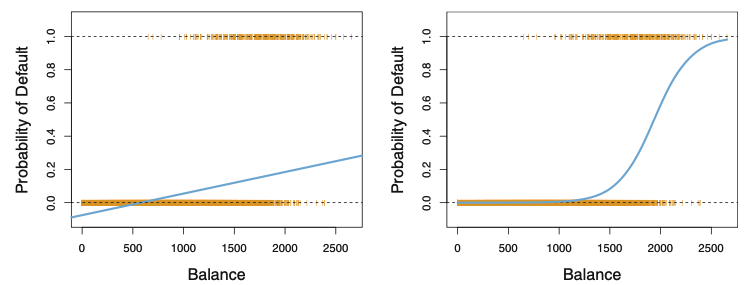
\includegraphics[width=0.6\textwidth]{fotos/14.png}
\caption{Clasificación usando los datos de Default. Izquierda: Probabilidad estimada de incumplimiento usando regresión lineal. ¡Algunas probabilidades estimadas son negativas! Las marcas naranjas indican los valores 0/1 codificados para incumplimiento (No o Sí). Derecha: Probabilidades predichas de incumplimiento usando regresión logística. Todas las probabilidades están entre 0 y 1.}
\label{fig:4.2}
\end{figure}

Para una respuesta binaria con una codificación 0/1 como la anterior, la regresión por mínimos cuadrados tiene sentido; se puede mostrar que el $\hat{X}\beta$ obtenido usando regresión lineal es de hecho una estimación de $\text{Pr}(\text{sobredosis de drogas} | X)$ en este caso especial. Sin embargo, si se usa regresión lineal, algunas de nuestras estimaciones podrían estar fuera del intervalo [0,1] (ver figura \ref{fig:4.2}), lo que las hace difíciles de interpretar como probabilidades. No obstante, las predicciones proporcionan un orden y pueden interpretarse como estimaciones de probabilidad crudas. Curiosamente, resulta que las clasificaciones que se obtienen si se usa regresión lineal para predecir una respuesta binaria serán las mismas que para el procedimiento de análisis discriminante lineal (LDA). \\

Sin embargo, el enfoque de variable ficticia no se puede extender fácilmente para acomodar respuestas cualitativas con más de dos niveles. Por estas razones, es preferible usar un método de clasificación que esté verdaderamente adaptado para valores de respuesta cualitativos, como los que se presentan a continuación.

\section{Regresión logística}

\subsection{Modelo logístico}

Veamos cómo se debe modelar la relación entre $p(X) = \Pr(Y = 1|X)$ y $X$ (por conveniencia se usará la codificación genérica 0/1 para la respuesta). Anteriormentese se habló de usar un modelo de regresión lineal para representar estas probabilidades:
\begin{equation}
p(X) = \beta_0 + \beta_1 X
\label{eq:4.1}
\end{equation}

Si se usa este enfoque para predecir default=Sí usando balance, entonces se obtiene el modelo mostrado en el panel izquierdo de la figura \ref{fig:4.2}. Cada vez que se ajusta una línea recta a una respuesta binaria que está codificada como 0 o 1, en principio siempre se puede predecir $p(X) < 0$ para algunos valores de $X$ y $p(X) > 1$ para otros (a menos que el rango de $X$ esté limitado). \\

Para evitar este problema, se debe modelar $p(X)$ usando una función que dé salidas entre 0 y 1 para todos los valores de $X$. Nótese que la frontera de decisión entre ambas salidas viene dada por $P(Y = 1 |X) = P(Y = 0 | X)$. Muchas funciones cumplen con esta descripción. En la regresión logística, se usa la función logística,
\begin{equation}
p(X) = \frac{e^{\beta_0 + \beta_1 X}}{1 + e^{\beta_0 + \beta_1 X}} = \frac{1}{1 + e^{-(\beta_0 + \beta_1 X)}}
\label{eq:4.2}
\end{equation}

Para ajustar el modelo (\ref{eq:4.2}), se usa un método llamado máxima verosimilitud, que se discute en la siguiente sección. El panel derecho de la figura \ref{fig:4.2} ilustra el ajuste del modelo de regresión logística a los datos de Default. Nótese que para balances bajos ahora se predice la probabilidad de incumplimiento como cercana a cero, pero nunca por debajo. Del mismo modo, para balances altos se predice una probabilidad de incumplimiento cercana a uno, pero nunca por encima. Después de manipular un poco (\ref{eq:4.2}), se encuentra que
\begin{equation}
\frac{p(X)}{1 - p(X)} = e^{\beta_0 + \beta_1 X}
\label{eq:4.3}
\end{equation}

La cantidad $\frac{p(X)}{1 - p(X)}$ se llama las probabilidades (\textit{odds}), y puede tomar cualquier valor entre 0 e $\infty$. Valores de las probabilidades cercanos a 0 e $\infty$ indican probabilidades muy bajas y muy altas de incumplimiento, respectivamente. Al tomar el logaritmo de ambos lados de (\ref{eq:4.3}), se llega a
\begin{equation}
\log\left(\frac{p(X)}{1 - p(X)}\right) = \beta_0 + \beta_1 X
\label{eq:4.4}
\end{equation}

La transformación monótona del lado izquierdo se llama el logaritmo de las probabilidades (\textit{log-odds}) o \textit{logit}. Se ve que el modelo de regresión logística (\ref{eq:4.2}) tiene un \textit{logit} que es lineal en $X$. \\

En un modelo de regresión lineal, $\beta_1$ da el cambio promedio en $Y$ asociado con un aumento de una unidad en $X$. En contraste, en un modelo de regresión logística, aumentar $X$ en una unidad cambia el logaritmo de las probabilidades en $\beta_1$ (\ref{eq:4.4}) o, equivalentemente, multiplica las probabilidades por $e^{\beta_1}$ (\ref{eq:4.3}). Sin embargo, debido a que la relación entre $p(X)$ y $X$ en (\ref{eq:4.2})) no es una línea recta, $\beta_1$ no corresponde al cambio en $p(X)$ asociado con un aumento de una unidad en $X$. La cantidad que $p(X)$ cambia debido a un cambio de una unidad en $X$ dependerá del valor actual de $X$. Pero independientemente del valor de $X$, si $\beta_1$ es positivo, entonces aumentar $X$ estará asociado con un aumento en $p(X)$, y si $\beta_1$ es negativo, entonces aumentar $X$ estará asociado con una disminución en $p(X)$.

\subsection{Estimación de los coeficientes}

Los coeficientes $\beta_0$ y $\beta_1$ en (\ref{eq:4.2}) son desconocidos y deben ser estimados basándose en los datos de entrenamiento disponibles. Aunque se podría usar mínimos cuadrados (no lineales) para ajustar el modelo (\ref{eq:4.4}), el método de máxima verosimilitud es preferible, ya que tiene mejores propiedades estadísticas. La intuición básica detrás del uso de máxima verosimilitud para ajustar un modelo de regresión logística es la siguiente: se intenta encontrar $\hat{\beta}_0$ y $\hat{\beta}_1$ de manera que al insertar estas estimaciones en el modelo para $p(X)$, dado en (\ref{eq:4.2}), se obtenga un número cercano a uno para todos los individuos que cumplieron, y un número cercano a cero para todos los individuos que incumplieron. Esta intuición se puede formalizar usando una ecuación matemática llamada función de verosimilitud:
\begin{equation}
\ell(\beta_0, \beta_1) = \prod_{i:y_i=1}^n p(x_i) \prod_{i':y_{i'} = 0} (1 - p(x_{i'}))
\label{eq:4.5}
\end{equation}

Las estimaciones $\hat{\beta}_0$ y $\hat{\beta}_1$ se eligen para maximizar esta función de verosimilitud. En el contexto de la regresión lineal, el enfoque de mínimos cuadrados es de hecho un caso especial de máxima verosimilitud. \\

Muchos aspectos de la salida de la regresión logística son similares a la salida de la regresión lineal. Por ejemplo, se puede medir la precisión de las estimaciones de los coeficientes calculando sus errores estándar. El estadístico $z$ juega el mismo papel que el estadístico $t$ en la salida de la regresión lineal. Por ejemplo, el estadístico $z$ asociado con $\hat{\beta}_1$ es igual a $\hat{\beta}_1 / SE(\hat{\beta}_1)$, por lo que un valor grande (absoluto) del estadístico $z$ indica evidencia en contra de la hipótesis nula $H_0: \beta_1 = 0$. Esta hipótesis nula implica que $p(X) = \frac{e^{\beta_0}}{1 + e^{\beta_0}}$, en otras palabras, que la probabilidad de incumplimiento no depende del balance. Si el valor $p$ asociado con balance es muy pequeño, se puede rechazar $H_0$. En otras palabras, se concluye que efectivamente hay una asociación entre balance y probabilidad de incumplimiento. \\

Una vez estimados los coeficientes, se pueden hacer predicciones de la probabilidad $\hat{p}(X)$ de forma sencilla 
\begin{equation}
\hat{p}(X) = \frac{1}{1 + e^{-(\hat{\beta}_0 + \hat{\beta}_1 X)}}
\label{eq:4.5.1}
\end{equation}

\subsection{Regresión logística múltiple}

Sea el problea de predecir una respuesta binaria usando múltiples predictores. La regresión logística anterior se puede generalizar de forma inmediata, de modo que el logarímto de las probabilidades serán
\begin{equation}
\log\left(\frac{p(X)}{1 - p(X)}\right) = \beta_0 + \beta_1 X_1 + \beta_2 X_2 + \dots + \beta_p X_p
\label{eq:4.6}
\end{equation}

\noindent y la probabilidad será 
\begin{equation}
p(X) = \frac{1}{1 + e^{-(\beta_0 + \beta_1 X_1 + \beta_2 X_2 + \dots + \beta_p X_p)}}
\label{eq:4.7}
\end{equation}

\subsection{Regresión logística no binaria}

Los modelos de regresión logística de binarios discutidos en las secciones anteriores tienen generalizaciones para múltiples clases, pero en la práctica no se utilizan con tanta frecuencia. Una de las razones es que el método que se discute en la próxima sección, el análisis discriminante, es popular para la clasificación de múltiples clases. 

\section{Análisis discriminante lineal}

La regresión logística implica modelar directamente $\Pr(Y = k | X = x)$ usando la función logística, dada por (\ref{eq:4.7}) para el caso de dos clases de respuesta. Se modela la distribución condicional de la respuesta $Y$, dado el(los) predictor(es) $X$. Ahora se considera un enfoque alternativo y menos directo para estimar estas probabilidades. En este enfoque alternativo (modelo generativo), se modela la distribución de los predictores $X$ por separado en cada una de las clases de respuesta (es decir, dado $Y$), y luego se usa el teorema de Bayes para convertir estas distribuciones en estimaciones de $\text{Pr}(Y = k | X = x)$. Cuando se asume que estas distribuciones son normales, resulta que el modelo es muy similar en forma a la regresión logística. Hay varias razones para usar un método distinto a la regresión logística (modelo discriminante):
\begin{itemize}
\item Cuando las clases están bien separadas, las estimaciones de los parámetros para el modelo de regresión logística son sorprendentemente inestables. El análisis discriminante lineal no sufre de este problema.
\item Si $n$ es pequeño y la distribución de los predictores $X$ es aproximadamente normal en cada una de las clases, el modelo de análisis discriminante lineal es nuevamente más estable que el modelo de regresión logística.
\item El análisis discriminante lineal es popular cuando se tienen más de dos clases de respuesta.
\end{itemize}

\subsection{Teorema de Bayes para clasificación}

\subsubsection{Regla de Bayes}

Sean dos eventos cualesquiera $A$ y $B$. La regla de Bayes establece que para encontrar $P(B | A)$ (probabilidad de que ocurra $B$ dado que $A$ ocurrió), se puede usar la siguiente relación:
\begin{equation}
P(B | A) = \frac{P (A \cap B)}{P(A)} = \frac{P(A | B)P(B)}{P(A)} 
\label{eq:4.8}
\end{equation}

\subsubsection{Regla de Bayes en problemas de clasificación}

Supongamos que se desea clasificar una observación en una de $K$ clases distintas, donde $K \geq 2$, es decir, la variable de respuesta cualitativa $Y$ puede tomar $K$ valores distintos y no ordenados. Sea $\pi_k$ la probabilidad general o \textit{a priori} de que una observación elegida al azar provenga de la $k$-ésima clase; esta es la probabilidad de que una observación dada esté asociada con la $k$-ésima categoría de la variable de respuesta $Y$. Sea $f_k(X) \equiv \text{Pr}(X = x | Y = k)$ la función de densidad de $X$ para una observación que proviene de la $k$-ésima clase. Así, $f_k(x)$ es relativamente grande si hay una alta probabilidad de que una observación en la $k$-ésima clase tenga $X \approx x$, y es pequeña si es muy improbable que una observación en la $k$-ésima clase tenga $X \approx x$. Entonces, el teorema de Bayes establece que
\begin{equation}
\Pr(Y = k | X = x) = \frac{P(X = x | Y = k) P (Y = k)}{P(X = x)} = \frac{\pi_k f_k(x)}{\sum_{l=1}^K \pi_l f_l(x)}
\label{eq:4.10}
\end{equation}

Se usará la abreviatura $p_k(X) = \Pr(Y = k | X = x)$. Esto sugiere que en lugar de calcular directamente $p_k(X)$, simplemente se pueden insertar estimaciones de $\pi_k$ y $f_k(X)$ en (\ref{eq:4.10}). En general, estimar $\pi_k$ es fácil si se tiene una muestra aleatoria de $Y$s de la población: simplemente se calcula la fracción de las observaciones de entrenamiento que pertenecen a la $k$-ésima clase. Sin embargo, estimar $f_k(X)$ tiende a ser más complicado, a menos que se asuman algunas formas simples para estas densidades. Se refiere a $p_k(x)$ como la probabilidad posterior de que una observación $X = x$ pertenezca a la $k$-ésima clase. Es decir, es la probabilidad de que la observación pertenezca a la $k$-ésima clase, dado el valor del predictor para esa observación. \\

Se sabe que el clasificador de Bayes, que clasifica una observación a la clase para la cual $p_k(X)$ es mayor, tiene la tasa de error más baja posible entre todos los clasificadores. (Esto, por supuesto, solo es cierto si los términos en (\ref{eq:4.10}) están todos especificados correctamente). Por lo tanto, si se puede encontrar una manera de estimar $f_k(X)$, entonces se puede desarrollar un clasificador que aproxime al clasificador de Bayes. Esto se verá en las próximas secciones.

\subsubsection{Análisis discriminante lineal para $p = 1$}

Por ahora, supongamos que $p = 1$, es decir, solo se tiene un predictor. Se desea obtener una estimación para $f_k(x)$ que se pueda insertar en (\ref{eq:4.10}) para estimar $p_k(x)$. Luego se clasificará una observación en la clase para la cual $p_k(x)$ sea mayor. Para estimar $f_k(x)$, primero se harán algunas suposiciones sobre su forma. \\

Supongamos que $f_k(x)$ es normal o gaussiana. En el entorno unidimensional, la densidad normal toma la forma
\begin{equation}
f_k(x) = \frac{1}{\sqrt{2\pi\sigma^2_k}} \exp\left(-\frac{(x - \mu_k)^2}{2\sigma^2_k}\right)
\label{eq:4.11}
\end{equation}

donde $\mu_k$ y $\sigma^2_k$ son los parámetros de media y varianza para la $k$-ésima clase. Por ahora, supongamos además que $\sigma^2_1 = \ldots = \sigma^2_K$, es decir, hay un término de varianza compartido entre todas las $K$ clases, que por simplicidad se puede denotar como $\sigma^2$. Insertando (\ref{eq:4.11}) en (\ref{eq:4.10}), se encuentra que
\begin{equation}
p_k(x) = \frac{\pi_k \frac{1}{\sqrt{2\pi\sigma^2}} \exp\left(-\frac{(x - \mu_k)^2}{2\sigma^2}\right)}{\sum_{l=1}^K \pi_l \frac{1}{\sqrt{2\pi\sigma^2}} \exp\left(-\frac{(x - \mu_l)^2}{2\sigma^2}\right)}
\label{eq:4.12}
\end{equation}

Nótese que en (\ref{eq:4.12}), $\pi_k$ denota la probabilidad a priori de que una observación pertenezca a la $k$-ésima clase. El clasificador de Bayes implica asignar una observación $X = x$ a la clase para la cual (\ref{eq:4.12}) es mayor. Tomando el logaritmo de (\ref{eq:4.12}) y reorganizando los términos, no es difícil mostrar que esto es equivalente a asignar la observación a la clase para la cual
\begin{equation}
\delta_k(x) = x \frac{\mu_k}{\sigma^2} - \frac{\mu_k^2}{2\sigma^2} + \log(\pi_k)
\label{eq:4.13}
\end{equation}

es mayor. Por ejemplo, si $K = 2$ y $\pi_1 = \pi_2$, entonces el clasificador de Bayes asigna una observación a la clase 1 si $2x(\mu_1 - \mu_2) > \mu_2^2 - \mu_1^2$, y a la clase 2 en caso contrario. En este caso, la frontera de decisión de Bayes corresponde al punto donde
\begin{equation}
x = \frac{\mu_1^2 - \mu_2^2}{2(\mu_1 - \mu_2)} = \frac{\mu_1 + \mu_2}{2}
\label{eq:4.14}
\end{equation}

\begin{figure}[h]
\centering
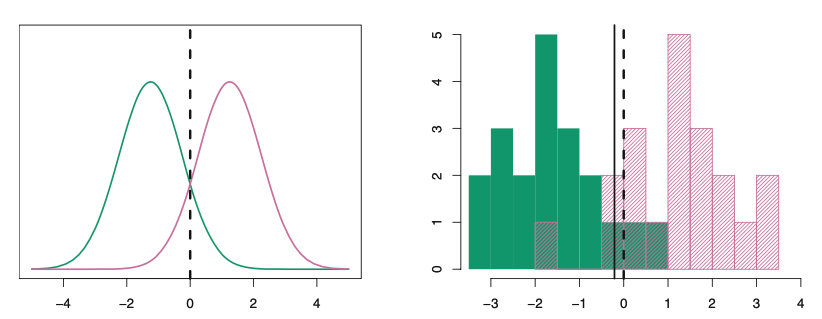
\includegraphics[width=0.7\textwidth]{fotos/15.png}
\caption{Izquierda: Se muestran dos funciones de densidad normal unidimensionales. La línea vertical discontinua representa la frontera de decisión de Bayes. Derecha: Se extrajeron 20 observaciones de cada una de las dos clases, y se muestran como histogramas. La frontera de decisión de Bayes se muestra nuevamente como una línea vertical discontinua. La línea vertical sólida representa la frontera de decisión LDA estimada a partir de los datos de entrenamiento.}
\label{fig:4.4}
\end{figure}

Un ejemplo se muestra en el panel izquierdo de la figura \ref{fig:4.4}. Las dos funciones de densidad normal que se muestran, $f_1(x)$ y $f_2(x)$, representan dos clases distintas. Los parámetros de media y varianza para las dos funciones de densidad son $\mu_1 = -1.25$, $\mu_2 = 1.25$, y $\sigma^2_1 = \sigma^2_2 = 1$. Las dos densidades se superponen, por lo que dado que $X = x$, hay cierta incertidumbre sobre la clase a la que pertenece la observación. Si se asume que una observación es igualmente probable que provenga de cualquiera de las dos clases, es decir, $\pi_1 = \pi_2 = 0.5$, entonces al inspeccionar (\ref{eq:4.14}), se ve que el clasificador de Bayes asigna la observación a la clase 1 si $x < 0$ y a la clase 2 en caso contrario. \\

Nótese que en este caso, se puede calcular el clasificador de Bayes porque se sabe que $X$ se extrae de una distribución gaussiana dentro de cada clase, y se conocen todos los parámetros involucrados. En una situación de la vida real, no se puede calcular el clasificador de Bayes. En la práctica, incluso si se está bastante seguro de la suposición de que $X$ se extrae de una distribución gaussiana dentro de cada clase, aún se deben estimar los parámetros $\mu_1, \ldots, \mu_K$, $\pi_1, \ldots, \pi_K$, y $\sigma^2$. El método de análisis discriminante lineal (LDA) aproxima el clasificador de Bayes insertando estimaciones para $\pi_k$, $\mu_k$, y $\sigma^2$ en (\ref{eq:4.13}). En particular, se usan las siguientes estimaciones:
\begin{equation}
\hat{\mu}_k = \frac{1}{n_k} \sum_{i: y_i = k} x_i, \quad \hat{\sigma}^2 = \frac{1}{n - K} \sum_{k=1}^K \sum_{i: y_i = k} (x_i - \hat{\mu}_k)^2
\label{eq:4.15}
\end{equation}

donde $n$ es el número total de observaciones de entrenamiento, y $n_k$ es el número de observaciones de entrenamiento en la $k$-ésima clase. La estimación para $\mu_k$ es simplemente el promedio de todas las observaciones de entrenamiento de la $k$-ésima clase, mientras que $\hat{\sigma}^2$ se puede ver como un promedio ponderado de las varianzas muestrales para cada una de las $K$ clases. A veces se tiene conocimiento de las probabilidades de pertenencia a la clase $\pi_1, \ldots, \pi_K$, que se pueden usar directamente. En ausencia de cualquier información adicional, LDA estima $\pi_k$ usando la proporción de las observaciones de entrenamiento que pertenecen a la $k$-ésima clase. En otras palabras,
\begin{equation}
\hat{\pi}_k = \frac{n_k}{n}
\label{eq:4.16}
\end{equation}

El clasificador LDA inserta las estimaciones dadas en (\ref{eq:4.15}) y (\ref{eq:4.16}) en (\ref{eq:4.13}), y asigna una observación $X = x$ a la clase para la cual
\begin{equation}
\hat{delta}_k(x) = x \frac{\hat{\mu}_k}{\hat{\sigma}^2} - \frac{\hat{\mu}_k^2}{2\hat{\sigma}^2} + \log(\hat{\pi}_k)
\label{eq:4.17}
\end{equation}

es mayor. La palabra "lineal" en el nombre del clasificador proviene del hecho de que las funciones discriminantes $\hat{\delta}_k(x)$ en (\ref{eq:4.17}) son funciones lineales de $x$ (en lugar de una función más compleja de $x$). \\

El panel derecho de la figura \ref{fig:4.4} muestra un histograma de una muestra aleatoria de 20 observaciones de cada clase. Para implementar LDA, se comenzó estimando $\pi_k$, $\mu_k$, y $\sigma^2$ usando (\ref{eq:4.15}) y (\ref{eq:4.16}). Luego se calculó la frontera de decisión, mostrada como una línea sólida negra, que resulta de asignar una observación a la clase para la cual (\ref{eq:4.17}) es mayor. Todos los puntos a la izquierda de esta línea se asignarán a la clase verde, mientras que los puntos a la derecha de esta línea se asignarán a la clase púrpura. En este caso, dado que $n_1 = n_2 = 20$, se tiene $\hat{\pi}_1 = \hat{\pi}_2$. Como resultado, la frontera de decisión corresponde al punto medio entre las medias muestrales para las dos clases, $(\hat{\mu}_1 + \hat{\mu}_2)/2$. La figura indica que la frontera de decisión LDA está ligeramente a la izquierda de la frontera de decisión óptima de Bayes, que en cambio es igual a $(\mu_1 + \mu_2)/2 = 0$. Dado que estos son datos simulados, se puede generar un gran número de observaciones de prueba para calcular la tasa de error de Bayes y la tasa de error de prueba de LDA. Estas son 10.6\% y 11.1\%, respectivamente. En otras palabras, la tasa de error del clasificador LDA es solo 0.5\% por encima de la tasa de error más baja posible. Esto indica que LDA está funcionando bastante bien en este conjunto de datos. \\

En resumen, el clasificador LDA resulta de suponer que las observaciones dentro de cada clase provienen de una distribución normal con un vector de media específico de la clase y una varianza común $\sigma^2$, e insertar estimaciones para estos parámetros en el clasificador de Bayes. Más adelante, se considerará un conjunto de suposiciones menos estrictas, permitiendo que las observaciones en la $k$-ésima clase tengan una varianza específica de la clase, $\sigma^2_k$.

\subsubsection{Análisis discriminante lineal para $p > 1$}

Para extender el clasificador LDA al caso de múltiples predictores, se asume que $X = (X_1, X_2, \ldots, X_p)$ se extrae de una distribución gaussiana multivariante (o normal multivariante), con un vector de media específico de la clase y una matriz de covarianza común. \\

\begin{figure}[h]
\centering
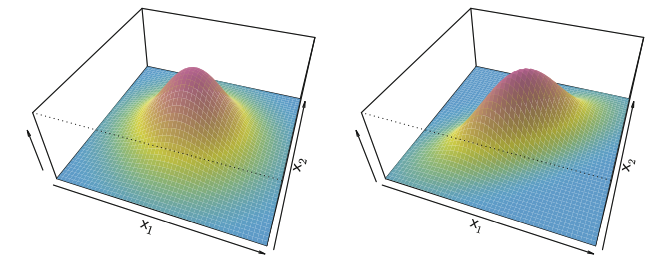
\includegraphics[width=0.7\textwidth]{fotos/16.png}
\caption{}
\label{fig:4.5}
\end{figure}

La distribución gaussiana multivariante asume que cada predictor individual sigue una distribución normal unidimensional, como en (\ref{eq:4.11}), con alguna correlación entre cada par de predictores. Dos ejemplos de distribuciones gaussianas multivariantes con $p = 2$ se muestran en la figura \ref{fig:4.5}. La altura de la superficie en cualquier punto particular representa la probabilidad de que tanto $X_1$ como $X_2$ caigan en una pequeña región alrededor de ese punto. La forma de campana se distorsionará si los predictores están correlacionados o tienen varianzas desiguales, como se ilustra en el panel derecho de la figura \ref{fig:4.5}. En esta situación, la base de la campana tendrá una forma elíptica, en lugar de circular. Para indicar que una variable aleatoria $p$-dimensional $X$ tiene una distribución gaussiana multivariante, escribimos $X \sim N(\mu, \Sigma)$. Aquí $E(X) = \mu$ es la media de $X$ (un vector con $p$ componentes), y $\text{Cov}(X) = \Sigma$ es la matriz de covarianza $p \times p$ de $X$. Formalmente, la densidad gaussiana multivariante se define como
\begin{equation}
f(x) = \frac{1}{(2\pi)^{p/2} |\Sigma|^{1/2}} \exp\left(-\frac{1}{2}(x - \mu)^T \Sigma^{-1} (x - \mu)\right)
\label{eq:4.18}
\end{equation}

En el caso de más de un predictor ($p > 1$), el clasificador LDA asume que las observaciones en la $k$-ésima clase se extraen de una distribución gaussiana multivariante $N(\mu_k, \Sigma)$, donde $\mu_k$ es un vector de media específico de la clase, y $\Sigma$ es una matriz de covarianza común a todas las $K$ clases. Insertando la función de densidad para la $k$-ésima clase, $f_k(X = x)$, en (\ref{eq:4.10}) y realizando un poco de álgebra, se revela que el clasificador de Bayes asigna una observación $X = x$ a la clase para la cual
\begin{equation}
\delta_k(x) = x^T \Sigma^{-1} \mu_k - \frac{1}{2} \mu_k^T \Sigma^{-1} \mu_k + \log(\pi_k)
\label{eq:4.19}
\end{equation}

\noindent es mayor. Esta es la versión vector/matriz de (\ref{eq:4.13}). \\

\begin{figure}[h]
\centering
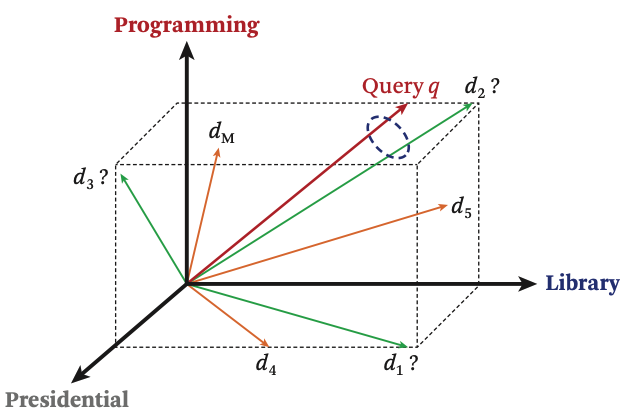
\includegraphics[width=0.7\textwidth]{fotos/17.png}
\caption{}
\label{fig:4.6}
\end{figure}

Un ejemplo se muestra en el panel izquierdo de la figura \ref{fig:4.6}. Se muestran tres clases gaussianas de igual tamaño con vectores de media específicos de la clase y una matriz de covarianza común. Las tres elipses representan regiones que contienen el 95\% de la probabilidad para cada una de las tres clases. Las líneas discontinuas son las fronteras de decisión de Bayes. En otras palabras, representan el conjunto de valores $x$ para los cuales $\delta_k(x) = \delta_\ell(x)$; es decir,
\begin{equation}
x^T \Sigma^{-1} \mu_k - \frac{1}{2} \mu_k^T \Sigma^{-1} \mu_k = x^T \Sigma^{-1} \mu_\ell - \frac{1}{2} \mu_\ell^T \Sigma^{-1} \mu_\ell
\label{eq:4.20}
\end{equation}

\noindent que puede reescribirse como
\begin{equation}
x^T \Sigma^{-1} (\mu_k - \mu_\ell) = \frac{1}{2} (\mu_k^T \Sigma^{-1} \mu_k - \mu_\ell^T \Sigma^{-1} \mu_\ell)
\label{eq:4.20.1}
\end{equation}

para $k \neq l$. (El término $\log(\pi_k)$ de (\ref{eq:4.19}) ha desaparecido porque cada una de las tres clases tiene el mismo número de observaciones de entrenamiento; es decir, $\pi_k$ es el mismo para cada clase). Nótese que hay tres líneas que representan las fronteras de decisión de Bayes porque hay tres pares de clases entre las tres clases. Es decir, una frontera de decisión de Bayes separa la clase 1 de la clase 2, una separa la clase 1 de la clase 3, y una separa la clase 2 de la clase 3. Estas tres fronteras de decisión de Bayes dividen el espacio de predictores en tres regiones. El clasificador de Bayes clasificará una observación según la región en la que se encuentre. \\

Una vez más, se necesita estimar los parámetros desconocidos $\mu_1, \ldots, \mu_K$, $\pi_1, \ldots, \pi_K$, y $\Sigma$; las fórmulas son similares a las utilizadas en el caso unidimensional, dadas en (\ref{eq:4.15}). Para asignar una nueva observación $X = x$, LDA inserta estas estimaciones en (\ref{eq:4.19}) y clasifica a la clase para la cual $\hat{\delta}_k(x)$ es mayor. Nótese que en (\ref{eq:4.19}) $\delta_k(x)$ es una función lineal de $x$; es decir, la regla de decisión LDA depende de $x$ solo a través de una combinación lineal de sus elementos. Una vez más, esta es la razón del término ``lineal'' en LDA. \\

En el panel derecho de la figura \ref{fig:4.6}, se muestran 20 observaciones extraídas de cada una de las tres clases, y las fronteras de decisión LDA resultantes se muestran como líneas negras sólidas. En general, las fronteras de decisión LDA están bastante cerca de las fronteras de decisión de Bayes, mostradas nuevamente como líneas discontinuas. Las tasas de error de prueba para los clasificadores de Bayes y LDA son 0.0746 y 0.0770, respectivamente. Esto indica que LDA está funcionando bien en estos datos. Las tasas de error de entrenamiento suelen ser más bajas que las tasas de error de prueba, que son la cantidad real de interés. La razón es que se ajustan específicamente los parámetros de nuestro modelo para que funcionen bien en los datos de entrenamiento. Cuanto mayor sea la relación de parámetros $p$ con el número de muestras $n$, más se espera que este sobreajuste juegue un papel. \\

En la práctica, un clasificador binario como este puede cometer dos tipos de errores: puede asignar incorrectamente a un individuo que incumple a la categoría de no incumplimiento, o puede asignar incorrectamente a un individuo que no incumple a la categoría de incumplimiento. A menudo es de interés determinar cuál de estos dos tipos de errores se están cometiendo. Una matriz de confusión es una forma conveniente de mostrar esta información. \\

LDA está tratando de aproximar el clasificador de Bayes, que tiene la tasa de error total más baja de todos los clasificadores (si el modelo gaussiano es correcto). Es decir, el clasificador de Bayes producirá el menor número posible de observaciones mal clasificadas, independientemente de la clase de la que provengan los errores. Algunos errores de clasificación resultarán de asignar incorrectamente a un cliente que no incumple a la clase de incumplimiento, y otros resultarán de asignar incorrectamente a un cliente que incumple a la clase de no incumplimiento. En contraste, una compañía de tarjetas de crédito podría desear particularmente evitar clasificar incorrectamente a un individuo que incumplirá, mientras que clasificar incorrectamente a un individuo que no incumplirá, aunque aún debe evitarse, es menos problemático. Es posible modificar LDA para desarrollar un clasificador que satisfaga mejor las necesidades de la compañía de tarjetas de crédito. \\

El clasificador de Bayes funciona asignando una observación a la clase para la cual la probabilidad posterior $p_k(X)$ es mayor. En el caso de dos clases, esto equivale a asignar una observación a la clase \textit{default} si
\begin{equation}
\Pr(\text{default = Yes} | X) > 0.5
\label{eq:4.21}
\end{equation}

Por lo tanto, el clasificador de Bayes, y por extensión LDA, usa un umbral del 50\% para la probabilidad posterior de \textit{default} para asignar una observación a la clase de incumplimiento. Sin embargo, si preocupa predecir incorrectamente el estado de incumplimiento para los individuos que incumplen, entonces se puede considerar bajar este umbral. Por ejemplo, se podría etiquetar a cualquier cliente con una probabilidad posterior de incumplimiento superior al 20\% a la clase de incumplimiento. En otras palabras, en lugar de asignar una observación a la clase \textit{default} si (\ref{eq:4.21}) se cumple, se podría asignar una observación a esta clase si
\begin{equation}
\Pr(\text{default = Yes} | X) > 0.2
\label{eq:4.22}
\end{equation}

Usar un umbral de 0.5, como en (\ref{eq:4.21}), minimiza la tasa de error general. Esto es de esperar, ya que el clasificador de Bayes usa un umbral de 0.5 y se sabe que tiene la tasa de error general más baja. Pero cuando se usa un umbral de 0.5, la tasa de error entre los individuos que incumplen es bastante alta (línea discontinua azul). A medida que se reduce el umbral, la tasa de error entre los individuos que incumplen disminuye constantemente, pero la tasa de error entre los individuos que no incumplen aumenta. \\

La curva ROC es un gráfico popular para mostrar simultáneamente los dos tipos de errores para todos los umbrales posibles. El nombre ``ROC'' es histórico y proviene de la teoría de comunicaciones. Es un acrónimo de características operativas del receptor. El rendimiento general de un clasificador, resumido en todos los umbrales posibles, se da por el área bajo la curva (AUC). Una curva ROC ideal abrazará la esquina superior izquierda, por lo que cuanto mayor sea el AUC, mejor será el clasificador. Se espera que un clasificador que no funcione mejor que el azar tenga un AUC de 0.5 (cuando se evalúa en un conjunto de prueba independiente no utilizado en el entrenamiento del modelo). Las curvas ROC son útiles para comparar diferentes clasificadores, ya que tienen en cuenta todos los umbrales posibles. \\

\begin{table}[h]
\centering
\begin{tabular}{c|c|c|c}
\hline
True class & \multicolumn{3}{c}{Clase predicha} \\ \hline
& $-$ o nulo & $+$ or no nulo & Total \\ \hline
$-$ o nulo & True Neg. (TN) & False Pos. (FP) & N \\ \hline
$+$ o no nulo & False Neg. (FN) & True Pos. (TP) & P \\ \hline
Total & N* & P* &  \\ \hline
\end{tabular}
\caption{Matriz de confusión. Posibles resultados al aplicar un clasificador a una población.}
\label{tb:4.6}
\end{table}

Variar el umbral del clasificador cambia su tasa de verdaderos positivos y su tasa de falsos positivos. Estas también se llaman la sensibilidad y uno menos la especificidad del clasificador. Dado que hay una variedad casi desconcertante de términos utilizados en este contexto, ahora damos un resumen. La tabla \ref{tb:4.6} muestra los posibles resultados al aplicar un clasificador (o prueba de diagnóstico) a una población. \\

\begin{table}[h]
\centering
\resizebox{\textwidth}{!}{
\begin{tabular}{c|c|c}
\hline
Nombre & Definición & Sinónimos \\ \hline
Tasa de verdaderos positivos & $TP/P$ & 1 - Error de tipo 2, sensibilidad, recall, probabilidad de detección \\ \hline
Tasa de falsos positivos & $FP/N$ & Error de tipo 1, 1 - especificidad \\ \hline
Valor predictivo positivo & $TP/P^*$ & Precisión, 1 - proporcion de falsos descumbrimientos \\ \hline
Valor predictivo negativo & $TN/N^*$ & \\ \hline
\end{tabular}
}
\caption{Medidas de rendimiento para clasificación.}
\label{tb:4.7}
\end{table}

La tabla \ref{tb:4.7} enumera muchas de las medidas de rendimiento populares que se utilizan en este contexto. Los denominadores para las tasas de falsos positivos y verdaderos positivos son los conteos de población reales en cada clase. En contraste, los denominadores para el valor predictivo positivo y el valor predictivo negativo son los conteos totales predichos para cada clase.

\subsubsection{Análisis discriminante cuadrático}

Como se ha discutido, LDA asume que las observaciones dentro de cada clase se extraen de una distribución gaussiana multivariante con un vector de media específico de la clase y una matriz de covarianza común a todas las $K$ clases. El análisis discriminante cuadrático (QDA) proporciona un enfoque alternativo. Al igual que LDA, el clasificador QDA resulta de asumir que las observaciones de cada clase se extraen de una distribución gaussiana, e insertar estimaciones para los parámetros en el teorema de Bayes para realizar la predicción. Sin embargo, a diferencia de LDA, QDA asume que cada clase tiene su propia matriz de covarianza. Es decir, asume que una observación de la $k$-ésima clase es de la forma $X \sim N(\mu_k, \Sigma_k)$, donde $\Sigma_k$ es una matriz de covarianza para la $k$-ésima clase. Bajo esta suposición, el clasificador de Bayes asigna una observación $X = x$ a la clase para la cual
\begin{align}
\delta_k(x) &= - \frac{1}{2} (x - \mu_k)^T \Sigma_k^{-1} (x - \mu_k) -\frac{1}{2} \log|\Sigma_k| + \log(\pi_k) \notag \\
&= - \frac{1}{2} x^T \Sigma_k^{-1} x + x^T \Sigma_k^{-1} \mu_k - \frac{1}{2} \mu_k^T \Sigma_k^{-1} \mu_k - \frac{1}{2} \log|\Sigma_k| + \log(\pi_k)
\label{eq:4.23}
\end{align}

es mayor. Entonces, el clasificador QDA implica insertar estimaciones para $\Sigma_k$, $\mu_k$, y $\pi_k$ en (\ref{eq:4.23}), y luego asignar una observación $X = x$ a la clase para la cual esta cantidad es mayor. A diferencia de (\ref{eq:4.19}), la cantidad $x$ aparece como una función cuadrática en (\ref{eq:4.23}). Aquí es donde QDA obtiene su nombre. \\

Elegir LDA o QDA radica en el equilibrio entre sesgo y varianza. Cuando hay $p$ predictores, estimar una matriz de covarianza requiere estimar $p(p+1)/2$ parámetros. QDA estima una matriz de covarianza separada para cada clase, para un total de $Kp(p+1)/2$ parámetros. Con 50 predictores, esto es un múltiplo de 1225, lo cual es una gran cantidad de parámetros. Al asumir en su lugar que las $K$ clases comparten una matriz de covarianza común, el modelo LDA se vuelve lineal en $x$, lo que significa que hay $Kp$ coeficientes lineales para estimar. En consecuencia, LDA es un clasificador mucho menos flexible que QDA, y por lo tanto tiene una varianza sustancialmente menor. Esto puede llevar potencialmente a un mejor rendimiento de predicción. Pero hay un compromiso: si la suposición de LDA de que las $K$ clases comparten una matriz de covarianza común es incorrecta, entonces LDA puede sufrir de alto sesgo. En términos generales, LDA tiende a ser una mejor opción que QDA si hay relativamente pocas observaciones de entrenamiento y por lo tanto reducir la varianza es crucial. En contraste, se recomienda QDA si el conjunto de entrenamiento es muy grande, de modo que la varianza del clasificador no sea una preocupación importante, o si la suposición de una matriz de covarianza común para las $K$ clases es claramente insostenible. \\

\begin{figure}[h]
\centering
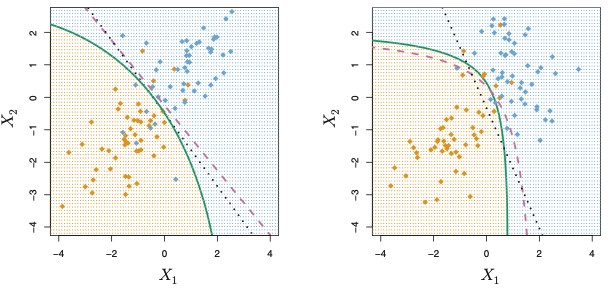
\includegraphics[width=0.7\textwidth]{fotos/18.png}
\caption{Izquierda: Las fronteras de decisión de Bayes (línea discontinua púrpura), LDA (línea punteada negra) y QDA (línea sólida verde) para un problema de dos clases con $\Sigma_1 = \Sigma_2$. El sombreado indica la regla de decisión de QDA. Dado que la frontera de decisión de Bayes es lineal, es más precisamente aproximada por LDA que por QDA. Derecha: Los detalles son los mismos que en el panel izquierdo, excepto que $\Sigma_1 \neq \Sigma_2$. Dado que la frontera de decisión de Bayes es no lineal, es más precisamente aproximada por QDA que por LDA.}
\label{fig:4.9}
\end{figure}

La figura \ref{fig:4.9} ilustra el rendimiento de LDA y QDA en dos escenarios. En el panel izquierdo, las dos clases gaussianas tienen una correlación común de 0.7 entre $X_1$ y $X_2$. Como resultado, la frontera de decisión de Bayes es lineal y es aproximada con precisión por la frontera de decisión de LDA. La frontera de decisión de QDA es inferior, porque sufre de mayor varianza sin una disminución correspondiente en el sesgo. En contraste, el panel derecho muestra una situación en la que la clase naranja tiene una correlación de 0.7 entre las variables y la clase azul tiene una correlación de $-0.7$. Ahora la frontera de decisión de Bayes es cuadrática, y por lo tanto QDA aproxima más precisamente esta frontera que LDA.